\documentclass[journal]{IEEEtran}

\usepackage{amsmath,amssymb}
\usepackage{array}
\usepackage{booktabs}
\usepackage{cite}
\usepackage{graphicx}
\usepackage{url}
\usepackage[hidelinks,bookmarksnumbered=true,bookmarksopen=true]{hyperref}
\usepackage{bookmark}

\graphicspath{{images/}{../figure/}}

\newcommand{\cmca}{CMCA}
\newcommand{\dacutmix}{DA-CutMix}
\newcommand{\ie}{i.e.,}
\newcommand{\eg}{e.g.,}

\begin{document}

\title{Cross-Modal Change Attention and Damage-Aware CutMix for Multimodal Building Damage Assessment}

\author{Hao Chen}

\maketitle

\pdfbookmark[1]{Abstract}{abstract}
\begin{abstract}
Multimodal building damage assessment requires reliable fusion between pre-event optical imagery and post-event synthetic aperture radar (SAR) observations, while also coping with severe damage-class imbalance and cross-event distribution shifts. This paper introduces a cross-modal change attention module and a damage-aware CutMix training strategy for all-weather building damage mapping. The method is designed as a lightweight plug-in for standard segmentation backbones and is evaluated through controlled ablation studies on the BRIGHT benchmark.
\end{abstract}

\begin{IEEEkeywords}
Building damage assessment, multimodal remote sensing, optical imagery, synthetic aperture radar, cross-modal attention, data augmentation, CutMix.
\end{IEEEkeywords}

\section{Introduction}
\label{sec:introduction}

% TODO: Write this section after the Methodology and Experiments sections are stable.
% A JSTARS-style introduction should motivate all-weather disaster response,
% summarize the optical/SAR fusion gap, identify cross-event generalization and
% damaged-class scarcity as the two main challenges, and then list the
% contributions of CMCA and DA-CutMix.

\section{Methodology}
\label{sec:methodology}

This section describes the proposed framework for multimodal building damage assessment. The method contains two complementary components: Cross-Modal Change Attention (\cmca), which improves optical/SAR feature fusion at the model level, and Damage-Aware CutMix (\dacutmix), which improves damage-class exposure and cross-event robustness at the data level. The overall technical roadmap is shown in Fig.~\ref{fig:roadmap}.

\begin{figure*}[!t]
    \centering
    
\includegraphics[width=\textwidth]{Technology Roadmap.png}
    \caption{Technical roadmap of the proposed multimodal building damage assessment framework. The pipeline contains architecture-level optical/SAR fusion through \cmca\ and data-level cross-event augmentation through \dacutmix.}
    \label{fig:roadmap}
\end{figure*}

\subsection{Problem Formulation}
\label{subsec:problem}

Given an aligned pre-event optical image $\mathbf{X}^{o}\in\mathbb{R}^{3\times H\times W}$ and a post-event SAR image $\mathbf{X}^{s}\in\mathbb{R}^{3\times H\times W}$, the objective is to predict a pixel-wise damage map
\begin{equation}
    \hat{\mathbf{Y}} = f_{\theta}(\mathbf{X}^{o}, \mathbf{X}^{s}),
\end{equation}
where $\hat{\mathbf{Y}}\in\{0,1,2,3\}^{H\times W}$. The four classes denote background, intact building, damaged building, and destroyed building, respectively. In the implementation, the SAR image is replicated to three channels and concatenated with the optical image, yielding a six-channel input. The network is trained for four-class semantic segmentation, while the binary localization label is obtained by merging the damaged and destroyed classes with the building class.

\subsection{Overall Framework}
\label{subsec:framework}

The baseline network processes the concatenated optical/SAR input using a standard segmentation backbone. In contrast, the proposed architecture separates the two modalities in the encoder and fuses them through \cmca\ at the deepest semantic level. Let $\mathbf{F}^{o}_{l}$ and $\mathbf{F}^{s}_{l}$ denote the optical and SAR features at encoder level $l$. Shallow skip features are fused by $1\times1$ convolutions,
\begin{equation}
    \mathbf{S}_{l} = \eta_{l}\left([\mathbf{F}^{o}_{l},\mathbf{F}^{s}_{l}]\right),
\end{equation}
where $[\cdot,\cdot]$ is channel-wise concatenation and $\eta_l(\cdot)$ is a learned projection. At the bottleneck level, \cmca\ estimates an explicit change-aware representation from optical-to-SAR cross-attention. The resulting change feature is concatenated with the original bottleneck features and passed to the decoder:
\begin{equation}
    \mathbf{F}_{b} = \psi\left([\mathbf{F}^{o}_{b},\mathbf{F}^{s}_{b},\mathbf{F}^{c}_{b}]\right),
\end{equation}
where $\mathbf{F}^{c}_{b}$ is the \cmca\ output and $\psi(\cdot)$ is implemented by a $1\times1$ convolution, batch normalization, and ReLU activation. This design keeps the decoder structure close to the original backbone while replacing simple early concatenation with explicit cross-modal comparison.

\begin{figure}[!t]
    \centering
    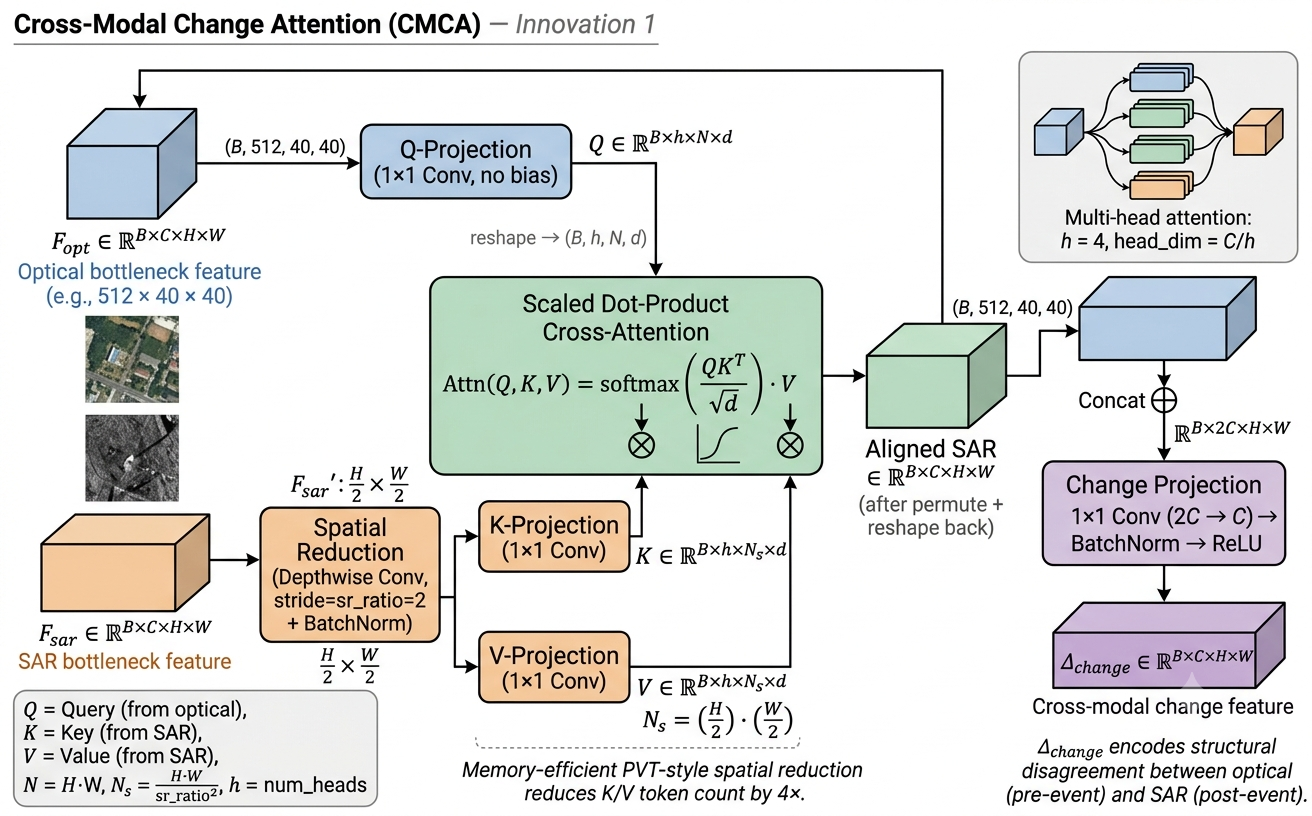
\includegraphics[width=\linewidth]{CMCA.png}
    \caption{Overview of the proposed Cross-Modal Change Attention module. Optical bottleneck features generate queries, while SAR bottleneck features generate keys and values after spatial reduction.}
    \label{fig:cmca}
\end{figure}

\subsection{Cross-Modal Change Attention}
\label{subsec:cmca}

Directly concatenating optical and SAR channels gives the network access to both modalities, but it does not force the model to learn where the post-event SAR response should be compared with the pre-event optical structure. \cmca\ addresses this limitation by using optical features as spatial queries and SAR features as keys and values.

Let $\mathbf{F}^{o}_{b},\mathbf{F}^{s}_{b}\in\mathbb{R}^{C\times h\times w}$ be the bottleneck features of the optical and SAR branches. First, \cmca\ projects the optical feature into queries and the SAR feature into keys and values:

\begin{equation}
    \begin{aligned}
    \mathbf{Q} &= W_{q}\mathbf{F}^{o}_{b}, \\
    \mathbf{K} &= W_{k}\mathcal{S}(\mathbf{F}^{s}_{b}), \\
    \mathbf{V} &= W_{v}\mathcal{S}(\mathbf{F}^{s}_{b})
    \end{aligned}
    \label{eq:qkv}
\end{equation}

where $W_q$, $W_k$, and $W_v$ are $1\times1$ convolutional projections. $\mathcal{S}(\cdot)$ is a depth-wise spatial reduction operator applied to keys and values for memory efficiency. In the current implementation, the spatial reduction ratio is set to 2.

For each attention head, the cross-modal attention map is computed as
\begin{equation}
    \mathbf{A} = \operatorname{softmax}
    \left(\frac{\mathbf{Q}\mathbf{K}^{\top}}{\sqrt{d}}\right),
\end{equation}
where $d$ is the head dimension. The SAR feature aligned to optical positions is then obtained by
\begin{equation}
    \tilde{\mathbf{F}}^{s}_{b} = \mathbf{A}\mathbf{V}.
\end{equation}
Finally, \cmca\ derives a change-enhanced feature by comparing the aligned SAR representation with the optical bottleneck feature:
\begin{equation}
    \mathbf{F}^{c}_{b} =
    \phi\left([\tilde{\mathbf{F}}^{s}_{b},\mathbf{F}^{o}_{b}]\right),
\end{equation}
where $\phi(\cdot)$ denotes a $1\times1$ convolution followed by batch normalization and ReLU. This formulation encourages high responses at locations where the post-event SAR structure is inconsistent with the pre-event optical building pattern, which is particularly useful for detecting severe structural damage.

The module is inserted only at the deepest encoder level. This placement reduces the quadratic cost of attention and allows the attention operation to focus on semantically rich building-level features. In the UNet implementation, both modality branches end with 512 channels, four attention heads are used, and the \cmca\ output is fused with the original optical and SAR bottleneck features before decoding.

\subsection{Damage-Aware CutMix}
\label{subsec:dacutmix}

Building damage assessment datasets are highly imbalanced: intact and background pixels dominate, while damaged and destroyed pixels are sparse. In addition, disaster events differ substantially in sensor response, urban structure, damage mechanism, and imaging geometry. To address these two issues at the data level, we introduce \dacutmix, an event-aware and damage-aware variant of CutMix for multimodal damage segmentation. The goal is not to synthesize physically realistic disaster scenes, but to break the shortcut correlation between an event-specific background and a damage label while increasing the exposure of rare damage classes.

Each training sample is represented as
\begin{equation}
    \mathcal{T}_{i} =
    \left(\mathbf{X}^{o}_{i}, \mathbf{X}^{s}_{i}, \mathbf{Y}_{i}, e_i\right),
\end{equation}
where $e_i$ is the disaster-event identifier parsed from the sample name. Standard geometric augmentation is first applied synchronously to the optical image, SAR image, and label map. For a target sample $\mathcal{T}_{i}$, \dacutmix\ is then attempted with probability $p$. A donor sample $\mathcal{T}_{j}$ is drawn from a different event, \ie, $e_j\neq e_i$, and undergoes the same type of synchronized geometric augmentation. A random rectangular box $B$ is drawn from the donor label map. The box is accepted only when it contains enough damage-class pixels:
\begin{equation}
    \sum_{\mathbf{u}\in B}
    \mathbb{I}\left[\mathbf{Y}_{j}(\mathbf{u})\in\mathcal{C}_{d}\right]
    \geq
    \max\left(n_{\min},\tau |B|\right),
    \label{eq:dacutmix_accept}
\end{equation}
where $\mathcal{C}_{d}=\{2,3\}$ corresponds to damaged and destroyed buildings, $n_{\min}$ is the minimum number of damage-class pixels, and $\tau$ is the minimum damage-class ratio. This rejection sampling does not require all pixels in $B$ to be damaged; the pasted patch can still contain background and intact buildings, preserving local context around the damage regions.

Let $\mathbf{M}_{B}$ be a binary mask that equals 1 inside the accepted box and 0 elsewhere. The mixed optical image, SAR image, and label map are generated jointly:
\begin{equation}
\label{eq:dacutmix_mix}
\begin{aligned}
    \tilde{\mathbf{X}}^{o} &=
    \mathbf{M}_{B}\odot\mathbf{X}^{o}_{j}
    +(1-\mathbf{M}_{B})\odot\mathbf{X}^{o}_{i}, \\
    \tilde{\mathbf{X}}^{s} &=
    \mathbf{M}_{B}\odot\mathbf{X}^{s}_{j}
    +(1-\mathbf{M}_{B})\odot\mathbf{X}^{s}_{i}, \\
    \tilde{\mathbf{Y}} &=
    \mathbf{M}_{B}\odot\mathbf{Y}_{j}
    +(1-\mathbf{M}_{B})\odot\mathbf{Y}_{i}.
\end{aligned}
\end{equation}
The same spatial box is pasted across optical, SAR, and label layers, preserving the pre-event optical, post-event SAR, and label alignment within the inserted donor patch. If no acceptable box is found after a fixed number of candidate boxes and donor samples, the original target crop is used unchanged. Unlike standard CutMix, the donor event constraint explicitly exposes the network to cross-event hybrids, while the damage-ratio constraint increases the frequency of informative damaged and destroyed regions. \dacutmix\ is used only during training; inference uses the original backbone without any additional operation or test-time cost.

\begin{figure}[!t]
    \centering
    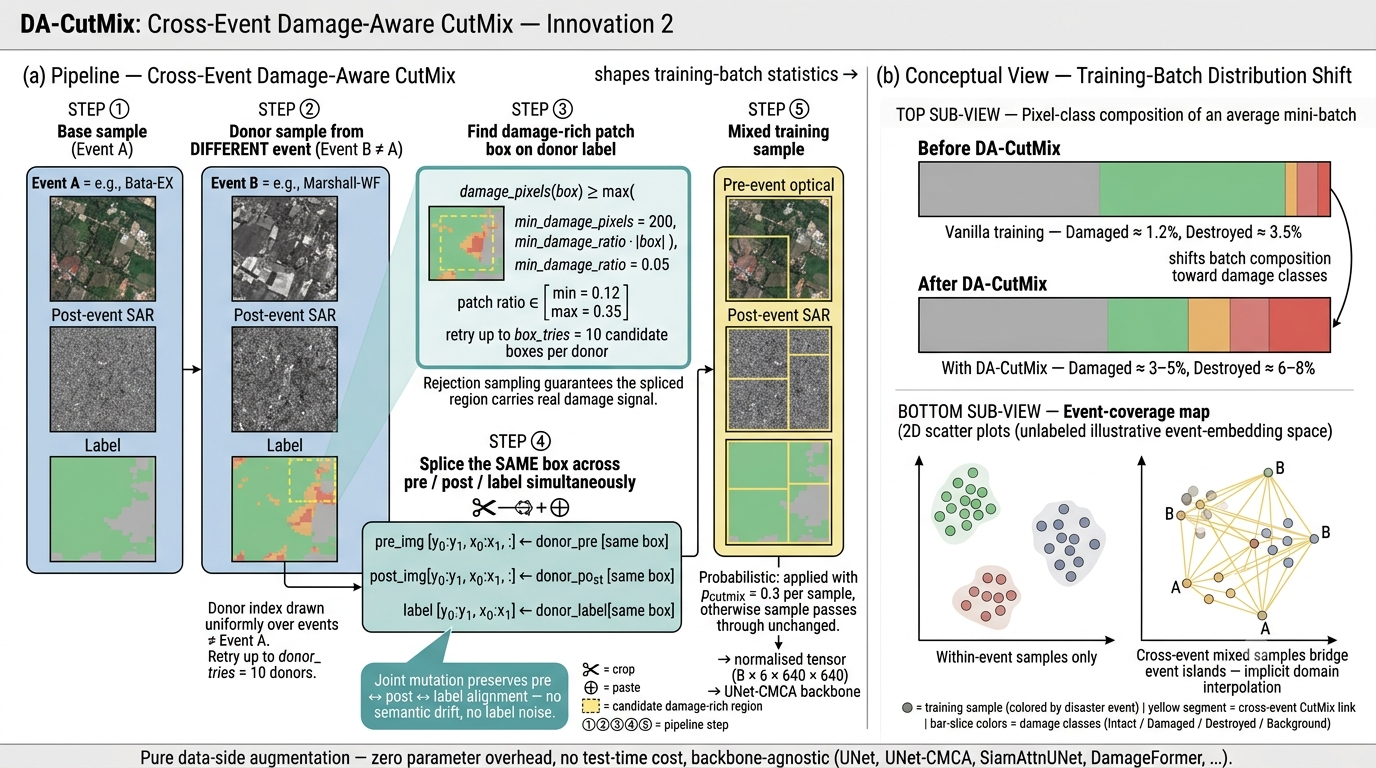
\includegraphics[width=\linewidth]{DA-CutMix.png}
    \caption{Training pipeline of \dacutmix. Donor patches are sampled from different disaster events and must contain a minimum amount of damaged or destroyed pixels before the same spatial box is pasted jointly into the optical image, SAR image, and label map.}
    \label{fig:dacutmix}
\end{figure}

\begin{figure*}[!t]
    \centering
    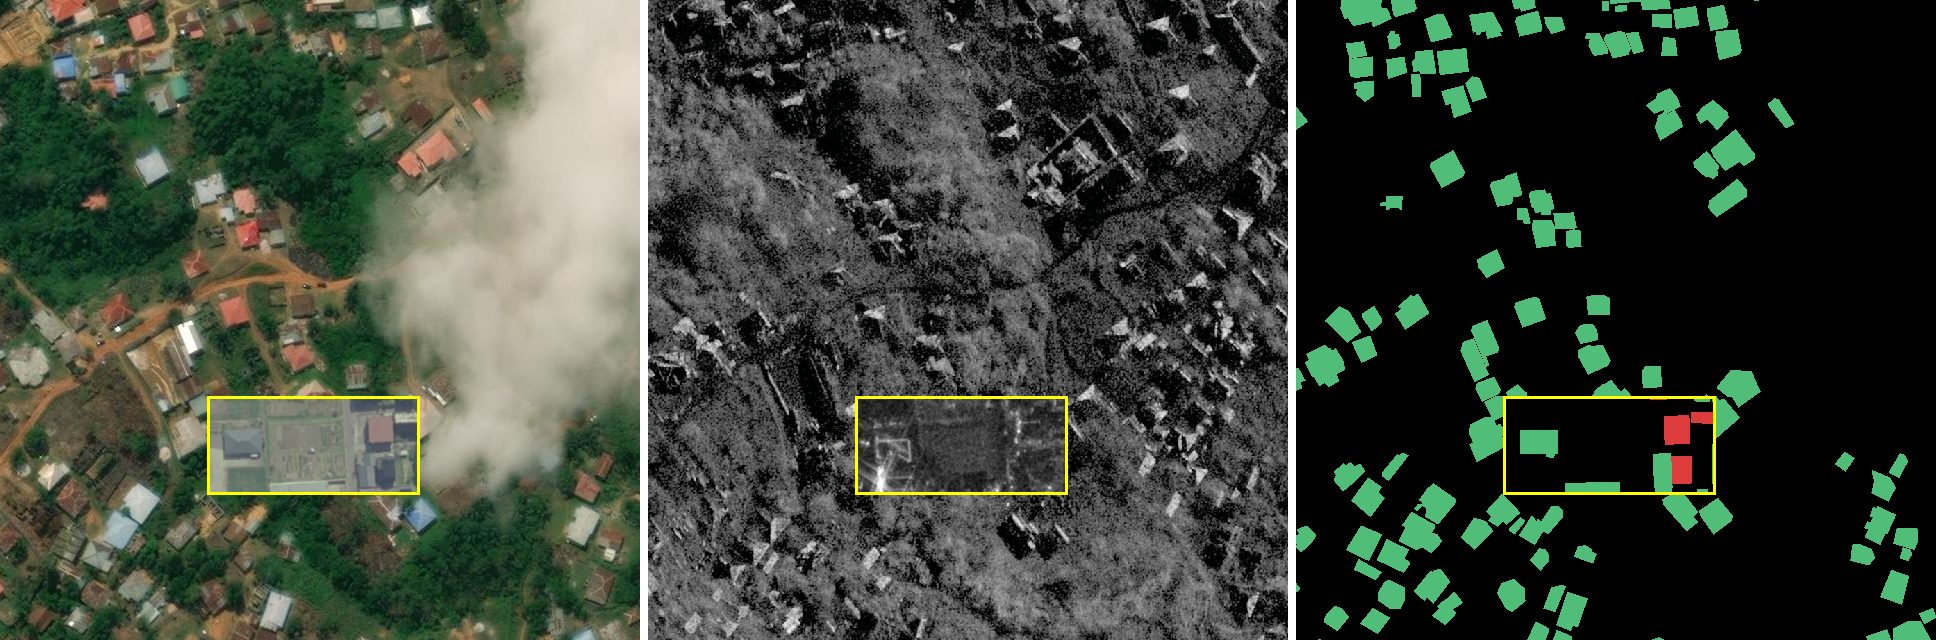
\includegraphics[width=0.86\textwidth]{dacutmix_example.png}
    \caption{Example \dacutmix\ training sample from the BRIGHT dataset. From left to right: pre-event optical image, post-event SAR image, and damage label map. The yellow rectangle denotes the same cross-event donor region pasted into all three layers, illustrating that \dacutmix\ preserves optical--SAR--label alignment while injecting a damage-rich patch.}
    \label{fig:dacutmix_example}
\end{figure*}

\subsection{Training Objective and Implementation Details}
\label{subsec:training}

The main segmentation objective combines pixel-wise cross-entropy with Lovasz-Softmax loss:
\begin{equation}
    \mathcal{L} =
    \mathcal{L}_{\mathrm{CE}}
    + 0.75\,\mathcal{L}_{\mathrm{Lovasz}}.
    \label{eq:training_loss}
\end{equation}
Unless otherwise stated, no auxiliary ordinal or contrastive losses are enabled for the \cmca\ and \dacutmix\ ablations.

The default training configuration follows the benchmark setting used in the implementation. Models are trained with AdamW using a learning rate of $1\times10^{-4}$ and a weight decay of $5\times10^{-3}$. The crop size is 640, the training batch size is 16, and the maximum training budget is 800,000 samples. For \dacutmix, the damage-class set is $\mathcal{C}_{d}=\{2,3\}$, $n_{\min}=200$, $\tau=0.05$, and up to 10 donor samples and 10 candidate boxes per donor are tested before falling back to the un-mixed target crop. The patch height and width are sampled independently between 0.12 and 0.35 of the crop size in the main runs, and the mixing probability is treated as a hyperparameter in the ablation study.

\section{Experiments and Results}
\label{sec:experiments}

\subsection{Dataset and Experimental Protocol}
\label{subsec:dataset_protocol}

Experiments are conducted on the BRIGHT multimodal building damage assessment benchmark. BRIGHT provides paired pre-event optical images, post-event SAR images, and pixel-level damage annotations. The annotations follow four semantic categories: background, intact building, damaged building, and destroyed building, as summarized in Table~\ref{tab:bright_label_definitions}. Following the standard supervised learning protocol in the benchmark code, the data are divided into 2917 training samples, 449 validation samples, and 877 test samples. The validation set is used for model selection, and the selected checkpoint is evaluated on the test set.

\begin{table}[!t]
\caption{Damage label definitions in the BRIGHT dataset.}
\label{tab:bright_label_definitions}
\centering
\footnotesize
\setlength{\tabcolsep}{3pt}
\renewcommand{\arraystretch}{1.1}
\begin{tabular}{>{\raggedright\arraybackslash}p{0.25\columnwidth}
                >{\raggedright\arraybackslash}p{0.68\columnwidth}}
\toprule
Category & Definition \\
\midrule
Background (0) & Non-building pixels. \\
Intact (1) & Building pixels without visible structural damage or apparent disaster-related surface changes. \\
Damaged (2) & Buildings with partial structural damage, such as missing roof components, visible cracks, partial wall or roof collapse, or surrounding hazard effects from water, mud, burning, or volcanic material. \\
Destroyed (3) & Buildings that are completely collapsed, burned, severely covered by water or mud, or no longer visible at the annotated location. \\
\bottomrule
\end{tabular}
\renewcommand{\arraystretch}{1.0}
\end{table}

\subsection{Evaluation Metrics}
\label{subsec:metrics}

We report overall accuracy (OA), mean intersection-over-union (mIoU), localization F1 score, classification F1 score, and per-class IoU. OA is computed over all pixels. For class $c$, IoU is defined as
\begin{equation}
    \mathrm{IoU}_{c} =
    \frac{\mathrm{TP}_{c}}
    {\mathrm{TP}_{c}+\mathrm{FP}_{c}+\mathrm{FN}_{c}},
\end{equation}
and mIoU is the average IoU over the four semantic classes. $F1_{\mathrm{loc}}$ evaluates binary building localization by merging intact, damaged, and destroyed buildings into a single foreground class. $F1_{\mathrm{clf}}$ is the harmonic mean of the F1 scores over the three building-related classes, namely intact, damaged, and destroyed. This metric places more emphasis on balanced damage recognition than on the dominant background class.

\subsection{Implementation Details}
\label{subsec:exp_implementation}

All methods use the same input format and data split. The pre-event optical image and post-event SAR image are concatenated into a six-channel tensor after synchronized geometric augmentation and normalization. Unless otherwise stated, models are trained for 800,000 samples with a crop size of 640, a batch size of 16, AdamW optimizer, learning rate $1\times10^{-4}$, and weight decay $5\times10^{-3}$. The loss function follows~\eqref{eq:training_loss}. For \dacutmix, donor patches are sampled from different disaster events with damaged-class set $\{2,3\}$, minimum damage pixels $n_{\min}=200$, minimum damage ratio $\tau=0.05$, and patch side length sampled from 0.12 to 0.35 of the crop size. The application probability $p$ is varied in the ablation study.

\subsection{Compared Variants}
\label{subsec:variants}

We evaluate the two proposed components under five representative segmentation backbones: UNet, DamageFormer, SiamAttnUNet, SiamCRNN, and DeepLabV3Plus. For each backbone, the baseline denotes the original model trained without \cmca\ or \dacutmix. The ``+\cmca'' setting replaces the original optical/SAR fusion with the proposed cross-modal attention module when the backbone architecture supports a paired-branch design. The ``+\dacutmix'' setting applies the proposed event-aware and damage-aware CutMix during training only. The ``+\cmca+\dacutmix'' setting combines the model-level and data-level components.

\subsection{Ablation Study}
\label{subsec:ablation}

Table~\ref{tab:overall_ablation} summarizes the overall ablation results on the standard test split. The table is organized by backbone so that the individual and combined effects of \cmca\ and \dacutmix\ can be compared under the same training protocol.

\begin{table*}[!t]
\caption{Overall Ablation Results on the BRIGHT Benchmark. Values Are Reported in Percentage.}
\label{tab:overall_ablation}
\centering
\scriptsize
\setlength{\tabcolsep}{2.6pt}
\renewcommand{\arraystretch}{0.96}
\begin{tabular}{lcccccccc}
\toprule
Method & F1$_{\mathrm{loc}}$ & F1$_{\mathrm{clf}}$ & OA & mIoU & Background & Intact & Damaged & Destroyed \\
\midrule
UNet & 88.32 & 70.91 & 95.52 & 64.74 & 96.28 & 71.62 & 37.48 & 53.59 \\
UNet + \dacutmix\ 0.25 & 88.65 & 70.18 & 95.54 & 64.44 & 96.28 & 72.36 & 36.27 & 52.84 \\
UNet + \dacutmix\ 0.30 & 88.07 & 70.89 & 95.48 & 64.46 & 96.22 & 71.43 & 38.05 & 52.15 \\
UNet + \cmca & 88.68 & \textbf{72.65} & 95.59 & 65.39 & 96.29 & 72.79 & \underline{39.30} & 53.20 \\
UNet + \cmca\ + \dacutmix\ 0.25 & \underline{89.09} & 72.03 & \textbf{95.82} & \underline{66.07} & \textbf{96.52} & \underline{73.29} & \textbf{40.53} & \underline{53.93} \\
UNet + \cmca\ + \dacutmix\ 0.30 & \textbf{89.18} & \underline{72.43} & \underline{95.81} & \textbf{66.16} & \underline{96.50} & \textbf{73.58} & 39.08 & \textbf{55.49} \\
\midrule
DamageFormer & 89.88 & 72.61 & 96.00 & 66.84 & 96.70 & 74.62 & 39.97 & 56.06 \\
DamageFormer + \dacutmix\ 0.25 & 89.91 & 72.25 & \underline{96.04} & 66.79 & \underline{96.75} & \underline{74.68} & 39.03 & \underline{56.70} \\
DamageFormer + \dacutmix\ 0.30 & \underline{89.94} & \underline{73.05} & \textbf{96.09} & \textbf{67.20} & \textbf{96.77} & \textbf{74.94} & \textbf{41.40} & 55.70 \\
DamageFormer + \cmca & 89.90 & 71.96 & 95.97 & 66.55 & 96.72 & 74.35 & 38.61 & 56.53 \\
DamageFormer + \cmca\ + \dacutmix\ 0.25 & \textbf{90.00} & 72.39 & 96.00 & 66.65 & 96.74 & 74.62 & 39.49 & 55.74 \\
DamageFormer + \cmca\ + \dacutmix\ 0.30 & 89.91 & \textbf{73.07} & 96.00 & \underline{67.14} & 96.71 & 74.54 & \underline{40.17} & \textbf{57.12} \\
\midrule
SiamAttnUNet & 88.26 & 71.79 & 95.51 & 65.03 & 96.21 & 72.06 & 38.24 & 53.60 \\
SiamAttnUNet + \dacutmix\ 0.25 & 88.03 & \underline{71.99} & 95.53 & 65.27 & 96.15 & 72.00 & \underline{39.08} & 53.83 \\
SiamAttnUNet + \dacutmix\ 0.30 & 87.92 & 71.85 & 95.49 & 65.28 & 96.11 & 71.95 & 37.45 & 55.62 \\
SiamAttnUNet + \cmca & \underline{88.60} & 71.51 & 95.56 & 64.81 & \underline{96.32} & 72.12 & 38.81 & 52.01 \\
SiamAttnUNet + \cmca\ + \dacutmix\ 0.25 & 88.21 & 71.59 & \underline{95.61} & \underline{65.71} & 96.26 & \underline{72.15} & 37.56 & \textbf{56.86} \\
SiamAttnUNet + \cmca\ + \dacutmix\ 0.30 & \textbf{88.77} & \textbf{72.88} & \textbf{95.71} & \textbf{66.26} & \textbf{96.39} & \textbf{72.87} & \textbf{39.95} & \underline{55.85} \\
\midrule
SiamCRNN & 89.11 & 72.12 & 95.83 & 66.13 & \underline{96.49} & 73.63 & \underline{40.22} & 54.17 \\
SiamCRNN + \dacutmix\ 0.25 & 89.05 & 72.15 & \underline{95.85} & 66.36 & \underline{96.49} & \underline{73.67} & 39.20 & \underline{56.09} \\
SiamCRNN + \dacutmix\ 0.30 & \textbf{89.30} & 72.29 & \textbf{95.87} & 66.33 & \textbf{96.55} & \textbf{73.79} & 39.62 & 55.38 \\
SiamCRNN + \cmca & 88.85 & \underline{72.85} & 95.75 & 66.25 & 96.42 & 73.12 & \textbf{41.26} & 54.21 \\
SiamCRNN + \cmca\ + \dacutmix\ 0.25 & 89.04 & \textbf{73.13} & 95.75 & \textbf{66.52} & 96.41 & 73.49 & 40.10 & 56.06 \\
SiamCRNN + \cmca\ + \dacutmix\ 0.30 & \underline{89.15} & 72.30 & 95.82 & \underline{66.50} & \underline{96.49} & 73.63 & 39.07 & \textbf{56.83} \\
\midrule
DeepLabV3Plus & 87.36 & 69.91 & 95.39 & 63.85 & 96.05 & 70.82 & 37.06 & 51.45 \\
DeepLabV3Plus + \dacutmix\ 0.25 & 87.68 & \textbf{71.77} & 95.53 & \underline{65.25} & 96.10 & 71.81 & \underline{39.80} & 53.30 \\
DeepLabV3Plus + \dacutmix\ 0.30 & 86.59 & 68.24 & 95.37 & 63.46 & 95.93 & 70.30 & 37.56 & 50.04 \\
DeepLabV3Plus + \cmca & 87.71 & 69.76 & 95.56 & 64.83 & 96.23 & 71.14 & 38.18 & \underline{53.76} \\
DeepLabV3Plus + \cmca\ + \dacutmix\ 0.25 & \textbf{88.79} & \underline{71.22} & \textbf{95.80} & \textbf{65.79} & \textbf{96.44} & \textbf{73.32} & 39.26 & \textbf{54.12} \\
DeepLabV3Plus + \cmca\ + \dacutmix\ 0.30 & \underline{88.45} & 70.87 & \underline{95.72} & 65.20 & \underline{96.36} & \underline{72.89} & \textbf{40.20} & 51.35 \\
\bottomrule
\end{tabular}
\renewcommand{\arraystretch}{1.0}
\end{table*}

For UNet, \cmca\ improves mIoU from 64.74\% to 65.39\%, with a notable gain of 1.82 percentage points on the damaged class. This indicates that explicit optical-to-SAR feature interaction helps the network recover damage-sensitive structural cues that are weakly exploited by direct channel concatenation. Standalone \dacutmix\ does not improve the UNet baseline in terms of mIoU, but it becomes effective when combined with \cmca. The best UNet setting, \cmca+\dacutmix\ with $p=0.30$, reaches 66.16\% mIoU, improving the baseline by 1.42 percentage points. It also improves $F1_{\mathrm{loc}}$ by 0.86 percentage points and $F1_{\mathrm{clf}}$ by 1.52 percentage points, suggesting that the combined method benefits both building localization and damage severity recognition.

DeepLabV3Plus provides another convolutional encoder--decoder baseline and shows a clear benefit from the proposed components. Standalone \dacutmix\ with $p=0.25$ improves mIoU from 63.85\% to 65.25\% and gives the highest $F1_{\mathrm{clf}}$ in this group. \cmca\ alone improves mIoU to 64.83\%, while the combined \cmca+\dacutmix\ setting with $p=0.25$ achieves the best mIoU of 65.79\%, corresponding to a 1.94-point gain over the baseline. This setting also gives the best $F1_{\mathrm{loc}}$, OA, background IoU, intact IoU, and destroyed-class IoU for DeepLabV3Plus. The $p=0.30$ combined setting instead gives the best damaged-class IoU, increasing it from 37.06\% to 40.20\%, which indicates that a larger mixing probability may favor harder damage pixels while slightly reducing destroyed-class consistency.

The stronger backbones reveal a more nuanced pattern. For DamageFormer, standalone \dacutmix\ with $p=0.30$ gives the best mIoU in this group, increasing mIoU from 66.84\% to 67.20\% and damaged-class IoU from 39.97\% to 41.40\%. The combined DamageFormer setting with $p=0.30$ does not exceed the standalone \dacutmix\ mIoU, but it achieves the best destroyed-class IoU in the group, improving it from 56.06\% to 57.12\%, and also gives the highest $F1_{\mathrm{clf}}$ of 73.07\%. This suggests that the two components may emphasize different damage categories depending on the backbone.

For SiamAttnUNet, the combined \cmca+\dacutmix\ setting with $p=0.30$ improves mIoU from 65.03\% to 66.26\% and raises $F1_{\mathrm{clf}}$ from 71.79\% to 72.88\%. It also improves damaged-class IoU by 1.71 percentage points. The $p=0.25$ combined setting gives the best destroyed-class IoU for this backbone, increasing it from 53.60\% to 56.86\%. For SiamCRNN, the baseline is already competitive, but the proposed components still improve damage recognition. \cmca\ alone raises damaged-class IoU from 40.22\% to 41.26\%, while \cmca+\dacutmix\ with $p=0.25$ gives the best mIoU and $F1_{\mathrm{clf}}$, reaching 66.52\% and 73.13\%, respectively. The $p=0.30$ combined setting gives the best destroyed-class IoU for SiamCRNN, improving it by 2.66 percentage points over the baseline.

\subsection{Per-Event Robustness}
\label{subsec:per_event}

We further inspect per-event mIoU to assess whether the gains are concentrated on a small number of events or distributed across disaster scenarios. In the UNet ablation, the \cmca+\dacutmix\ setting with $p=0.30$ obtains the best per-event mIoU on 10 out of the 15 evaluated events, and its average per-event gain over the UNet baseline is 3.50 percentage points. The $p=0.25$ combined setting is the best on four additional events, while standalone \cmca\ is best on one event. These results suggest that the proposed components are especially useful for improving event-level robustness rather than only optimizing the global pixel distribution.

The per-event behavior also shows that the optimal mixing probability is backbone-dependent. For DamageFormer, standalone \cmca\ gives the best event-level mIoU on five events and the \cmca+\dacutmix\ setting with $p=0.25$ is best on four events, even though standalone \dacutmix\ with $p=0.30$ gives the best global mIoU. For SiamAttnUNet, standalone \dacutmix\ with $p=0.30$ wins on five events, while \cmca\ and \cmca+\dacutmix\ with $p=0.25$ each win on three events. For SiamCRNN, \dacutmix\ with $p=0.30$ and \cmca+\dacutmix\ with $p=0.25$ each obtain the best result on four events. For DeepLabV3Plus, \cmca+\dacutmix\ with $p=0.25$ is the most stable event-level setting, winning on seven out of the 15 evaluated events and yielding an average per-event gain of 2.29 percentage points over the DeepLabV3Plus baseline. This observation motivates treating \dacutmix\ probability as a tunable training hyperparameter rather than a fixed constant.

\end{document}
